% DoseRAD2026 final submission — Task: PHOTON-MRI (single-task LNCS report, <=11 content pages).
\documentclass{llncs}
\usepackage{amsmath,amssymb,bm,mathtools}
\usepackage{graphicx,booktabs,array}
\usepackage[hidelinks]{hyperref}
\usepackage{tikz}
\usetikzlibrary{arrows.meta,positioning,fit,backgrounds}
\graphicspath{{figs/}}
\newcommand{\opS}{\mathcal{S}}\newcommand{\opD}{\mathcal{D}}\newcommand{\opX}{\mathcal{X}}
\newcommand{\opR}{\mathcal{R}}\newcommand{\opC}{\mathcal{C}}\newcommand{\gam}{\gamma}
\renewcommand{\topfraction}{.95}\renewcommand{\bottomfraction}{.6}
\renewcommand{\textfraction}{.05}\renewcommand{\floatpagefraction}{.75}
\setcounter{topnumber}{3}\setcounter{totalnumber}{5}

\begin{document}

\title{Dose-Aware MR-to-CT Synthesis through a Differentiable Physics-Prior Residual 3D U-Net
for Photon Dose Prediction on 0.35\,T MRI (DoseRAD2026 Photon-MRI Task)}
\titlerunning{Dose-Aware Synthesis for Photon-MRI Dose Prediction}
\author{Kai Wang \and Meixu Chen \and Rui Yang}
\authorrunning{K. Wang et al.}
\institute{Department of Radiation Oncology, University of Colorado Anschutz Medical Campus,
Aurora, CO, USA\\ \email{\{kai.2.wang,meixu.chen,ray.yang\}@cuanschutz.edu}}

\maketitle

\begin{abstract}
We predict photon control-point dose directly from 0.35\,T MRI by making synthetic-CT (sCT)
generation \emph{dose-aware}. A classifier--refiner synthesizer maps the MR to a density image;
an analytical, differentiable physics operator turns density and control point into six
dose-shaped channels; and a residual 3D U-Net corrects the analytical prior toward Monte Carlo.
Because the physics is differentiable in the density, the synthesizer is trained \emph{jointly
through it} with the dose loss; the sCT is optimized for the dose, not for image fidelity. This
matters: across five coarse-prior variants, standalone image quality did not predict fused dose
accuracy ($r{=}0.02$), and a TotalSegmentator-MRI lung mask with far better Dice than our
classifier gained nothing dosimetrically. The full chain lifts $\gam$1\%/1\,mm from 68.7
(bulk-density) through 82.6 (image-fidelity sCT) and 88.8 (dose-aware synthesis) to 90.7 (joint
training) on the development fold; 5-fold cross-validation gives $91.1\pm1.6$, and a
cross-validated real-CT ceiling of $95.8\pm1.3$ isolates the remaining synthesis cost at
$4.7\pm1.4$ points. On the hidden test set, MR intensity shift between training and test images
emerged as the dominant failure mode and was substantially mitigated by retraining the tissue
classifier with strong intensity-shift augmentation. The final full-data submission scored
$\gam$\,=\,84.11, per-beam MAE 0.0172, IDD 0.0127, DVH 1.00 at 94.8\,s per job; the fastest
runtime on the preliminary leaderboard at submission time.
\keywords{MR-only planning \and synthetic CT \and dose-aware synthesis \and differentiable
physics \and MR-linac}
\end{abstract}

\section{Introduction}
On MR-linacs and in MR-only workflows the planning image is an MRI, whose intensities encode
neither electron density nor attenuation. The established remedy (synthesize a CT, then compute
dose) optimizes the synthesis for an \emph{image} objective (MAE, SSIM, Dice) that is only a
surrogate for the clinically relevant quantity~\cite{mriproton,rsp,liver,ganbrain,uncert,dect}.
We instead couple synthesis and dose in one differentiable pipeline. An analytical physics
operator $\opC$ maps density and control-point descriptor to dose-shaped channels; a residual 3D
U-Net $\opD_\theta$ corrects the analytical prior toward Monte Carlo (MC); and because $\opC$ is
differentiable in the density, a synthesizer $\opX=\opR\circ\opS$ placed upstream is trained
\emph{through the physics} with the dose loss. The synthesizer is thereby free to place density
where the \emph{dose} needs it rather than where an image metric would reward it; and our
central empirical finding is that these two objectives genuinely diverge (Sec.~3.3). This report
details the Photon-MRI system; the same framework serves our submissions to all four DoseRAD2026
tasks.

\begin{figure}[t]\centering
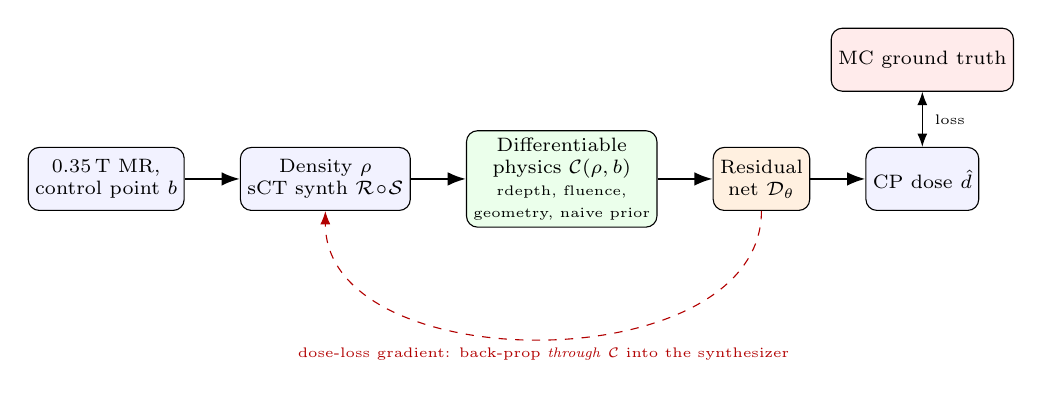
\begin{tikzpicture}[
 node distance=6mm and 7mm, >=Latex, font=\scriptsize,
 box/.style={draw, rounded corners, align=center, minimum height=8mm, inner sep=2.5pt, fill=blue!5},
 phys/.style={box, fill=green!8}, net/.style={box, fill=orange!12},
 every edge/.style={draw, ->, thick}]
\node[box] (img) {0.35\,T MR,\\ control point $b$};
\node[box, right=of img] (dens) {Density $\rho$\\ sCT synth $\opR\!\circ\!\opS$};
\node[phys, right=of dens] (chan) {Differentiable\\ physics $\opC(\rho,b)$\\ \tiny rdepth, fluence,\\ \tiny geometry, naive prior};
\node[net, right=of chan] (net) {Residual\\ net $\opD_\theta$};
\node[box, right=of net] (dose) {CP dose $\hat d$};
\node[box, above=7mm of dose, fill=red!8] (mc) {MC ground truth};
\draw (img) edge (dens) (dens) edge (chan) (chan) edge (net) (net) edge (dose);
\draw[<->] (dose) -- (mc) node[midway,right=1pt]{\tiny loss};
\draw[->, dashed, red!70!black] (net.south) to[out=-90,in=-90] node[midway,below,align=center]
 {\tiny dose-loss gradient: back-prop \emph{through} $\opC$ into the synthesizer} (dens.south);
\end{tikzpicture}
\caption{Dose-aware MR-only pipeline: the synthesizer is trained jointly through the
differentiable physics with the dose loss (dashed), so the sCT serves the dose, not an image
metric.}\label{fig:framework}
\end{figure}

\section{Methods}
\subsection{Data}
Official DoseRAD2026 training set~\cite{challenge} (75 patients: 39 thorax, 36 abdomen;
SynthRAD2025 cohort~\cite{synthrad}): per patient a co-registered 0.35\,T MR (ViewRay MRIdian,
bSSFP, breath-hold) and planning CT, beam parameters, and per-control-point MC dose-to-medium
(matRad~\cite{matrad}) on a $2{\times}2{\times}2$\,mm grid; 540 control points per patient. Per
the challenge definition, the MRI-task ground truth is the CT-computed MC dose mapped onto the
co-registered MR, so the achievable target for MR-only calculation is the CT dose itself; the
framing behind our real-CT-ceiling analysis (Sec.~3.3). The sCT refiner additionally uses 166
field-matched 0.35\,T MR--CT pairs from the public SynthRAD2025 pool (disjoint from validation
patients); no other external data. Development: 5-fold CV over all 75; \textbf{the final
submission is retrained on all 75}, with the leaderboard as held-out validation.

\subsection{Model}
\textbf{Synthesizer} $\opX=\opR\circ\opS$: $\opS$, a whole-image 3D U-Net classifier, assigns
each voxel to air/lung/soft-tissue/bone (CT-HU band edges $-500/-300/{+}200$) and maps classes
to a bulk-HU coarse CT; $\opR$, a whole-image refiner, maps $[\mathrm{MR},\mathrm{coarse}]$ to
the sCT, from which the official HU calibration yields density. \textbf{Physics} $\opC$: the six
photon channels (density, ray-marched radiological depth, MLC-projected primary fluence,
distance-to-CAX, source distance, naive analytical surrogate), all differentiable tensor
operations, with the per-ray skin-entry rule (depth accumulates from the first
$\rho>0.05$\,g/cm$^3$ crossing; prior masked strictly upstream). \textbf{Dose network}
$\opD_\theta$: DoseUNet3D (base 48; four levels; ASPP bottleneck; Softplus head; FiLM modality
conditioning), warm-started from the Photon-CT network. Figure~\ref{fig:chain} shows the full
deployed chain: synthesis quality and its dosimetric consequence in one figure.

\begin{figure}[t]\centering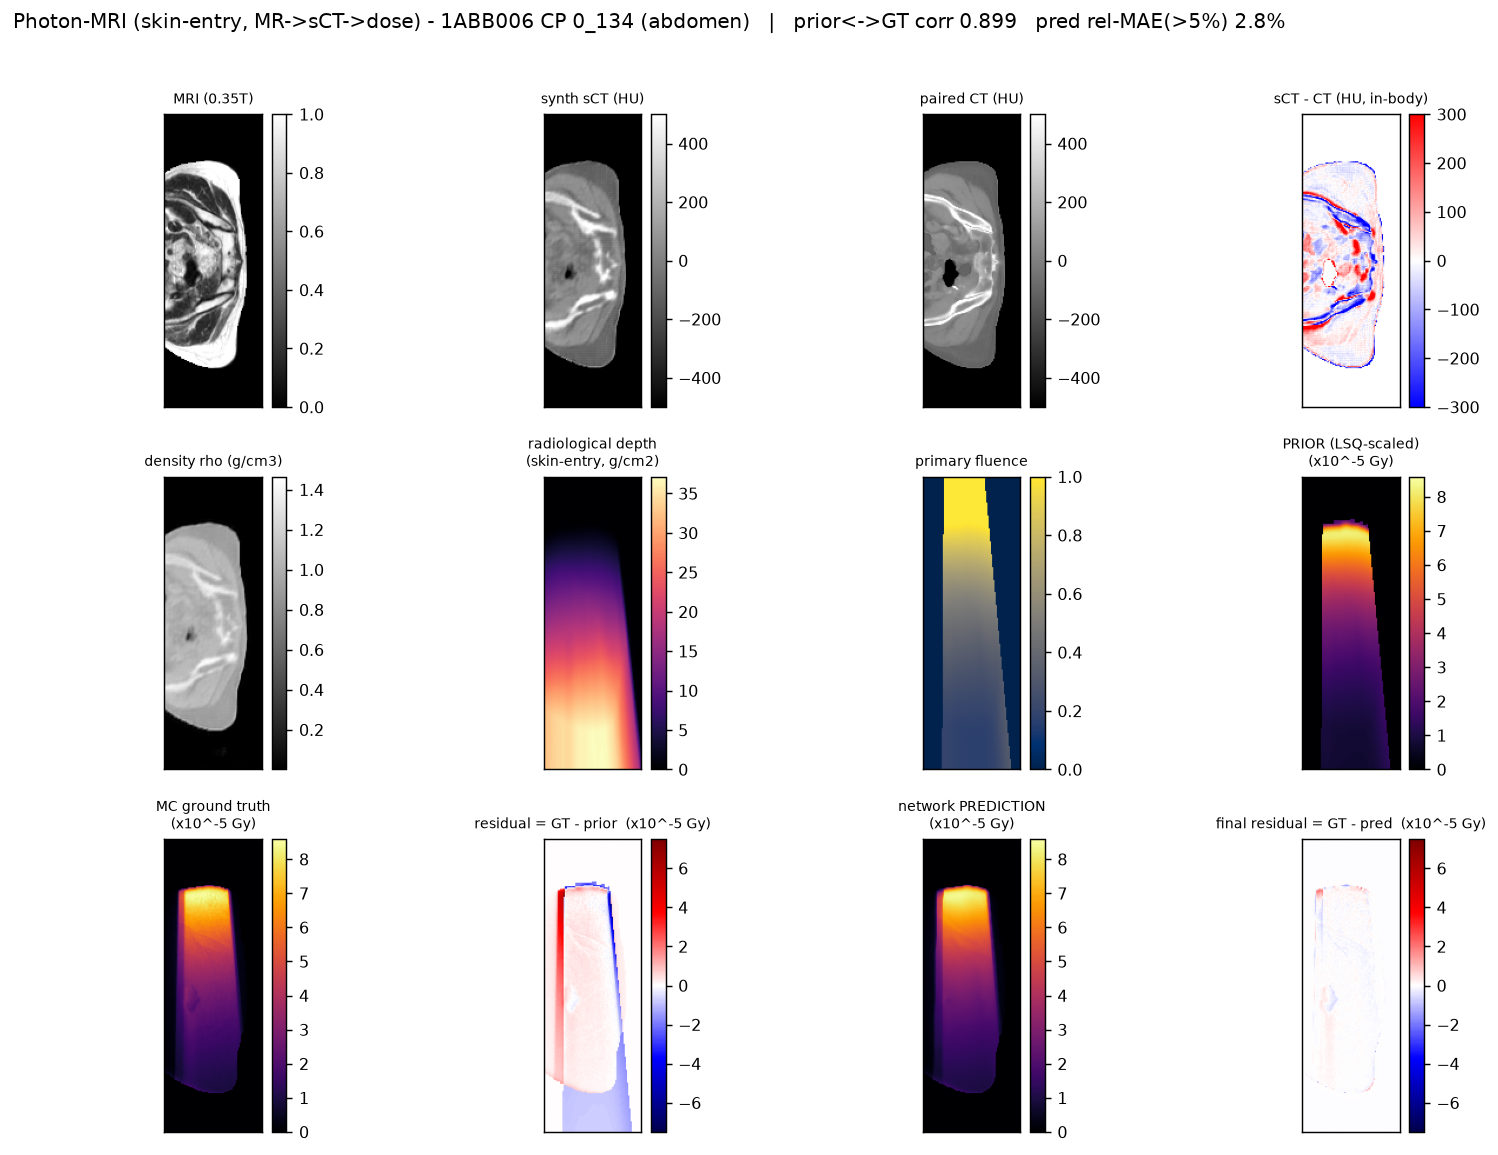
\includegraphics[width=\linewidth]{figS_residual_photonmri_abdomen.png}
\caption{Deployed Photon-MRI chain (abdomen, 1ABB006). Row 1: synthesis ; MR (0.35\,T) $\to$
synthetic CT $\to$ paired real CT $\to$ in-body sCT$-$CT residual. Remaining panels: physics
channels on the synthetic density $\to$ LSQ-scaled naive prior $\to$ MC ground truth $\to$
residual (GT$-$prior) $\to$ prediction $\to$ final residual (GT$-$pred).}\label{fig:chain}\end{figure}

\begin{figure}[t]\centering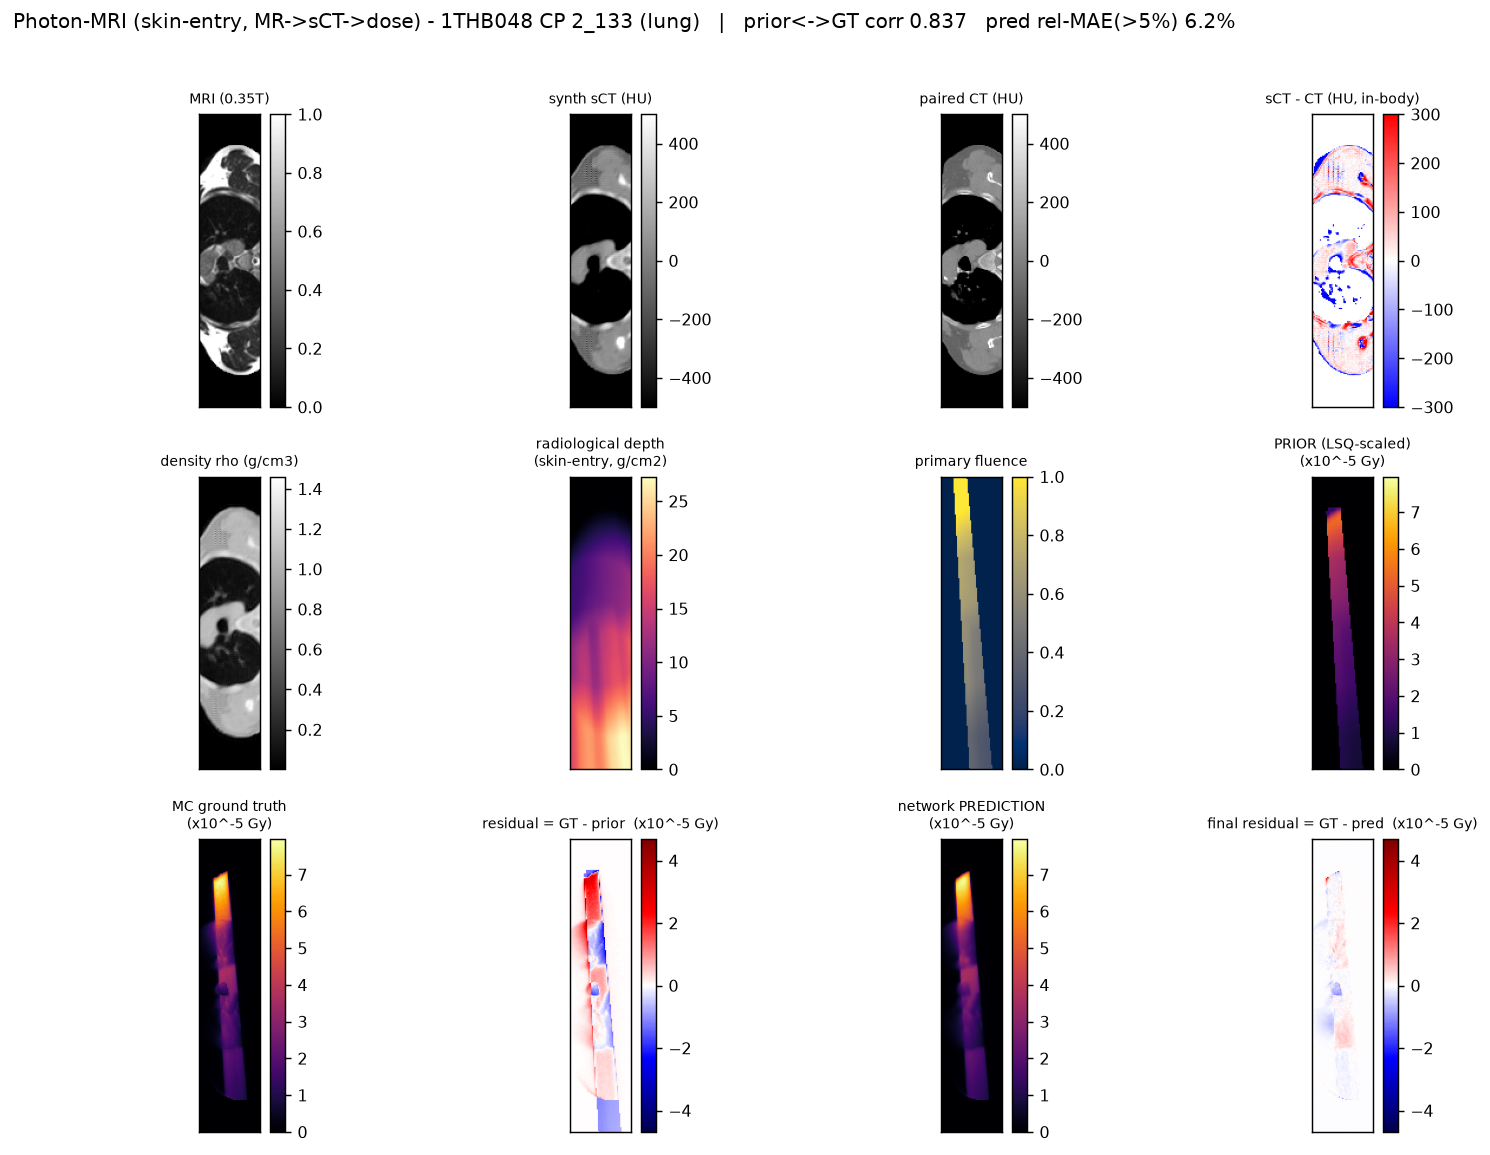
\includegraphics[width=\linewidth]{figS_residual_photonmri_lung.png}
\caption{As Fig.~\ref{fig:chain}, lung case: 0.35\,T MR carries little lung density
information; lung is the site of the largest synthesis cost.}\label{fig:chainlung}\end{figure}

\subsection{Training}
Stage 1: the tissue classifier and refiner are pretrained (the refiner also on the 166
field-matched pairs); the dose network is warm-started from Photon-CT. Stage 2 (dose-aware):
refiner and dose network train \emph{jointly}, 15--20k steps, with the dose loss
back-propagating through $\opC$ into the refiner, plus a region-weighted per-voxel sCT anchor to
the real CT as regularizer. Loss and optimization as in our CT system (high-dose-weighted $L_1$,
AdamW, EMA, patches $128^3$). \textbf{Robustness for the hidden test:} the dominant held-out
failure mode was MR \emph{intensity shift} between our training MRs and the hidden-test MRs
(diagnosed by leaderboard probes: internally synthesized shifts reproduced the drop, and the
shared tissue classifier accounted for most of it). The deployed classifier is therefore
retrained with strong MR intensity-shift augmentation (bias/gamma/scale perturbations); no
augmentation is used in dose training itself. Reproducibility: fixed seeds, YAML configs, EMA
checkpoints; code and weights to be open-sourced (Sec.~6).

\subsection{Evaluation}
Internal: plan-level local $\gam$~\cite{gamma} (pymedphys, 1\%/1\,mm, $\ge$10\% Rx cutoff,
byte-identical to the vendored official code), per-beam masked MAE, official IDD and
stratified-MAE reimplementations; a frozen 16-patient held-out cohort gates every deployment
change (\emph{no accuracy loss, no speed loss}). Mechanistic probes: the \emph{real-CT ceiling}
(the trained MRI pipeline re-run with the real CT substituted for the sCT, isolating the
synthesis cost patient-matched) and a five-variant coarse-prior sweep relating image fidelity to
fused dose accuracy. Runtime: official $T=t_{\rm fix}+N\cdot t_{\rm dose\,map}$, gate 181\,s,
double-weighted.

\section{Results}
\subsection{Accuracy: cross-validated and hidden-test}
Per-fold CV $\gam$1/1: 90.7/90.2/92.2/88.9/93.6 (mean $91.1\pm1.6$). Development fold ($n=16$):
$\gam$1/1 $=90.7\pm5.7$ (abdomen 94.6, lung 86.8), $\gam$2/2 $=97.7$, $\gam$3/3 $=99.1$;
per-beam masked MAE $1.55\pm0.38$\%. Table~\ref{tab:res} adds the hidden-test metrics. The
CV-to-hidden-test gamma drop ($91.1\to84.1$) is dominated by MR intensity shift (Sec.~2.3): on
the sister proton-MRI task the shift-augmented classifier recovered $+3.1$ board gamma, and the
same fix is deployed here.

\begin{table}[t]\centering
\caption{Photon-MRI results. CV: 5-fold over the 75 public patients. Hidden test: official
metrics of the final full-data submission (August 2026). Gate: 181\,s/job.}\label{tab:res}
\begin{tabular}{@{}lc@{}}\toprule
Metric & Value\\\midrule
CV plan $\gam$1\%/1\,mm (5-fold) & $91.1\pm1.6$\\
CV real-CT ceiling / synthesis cost & $95.8\pm1.3$ / $4.7\pm1.4$\\
Hidden-test per-beam masked MAE & $0.0172\pm0.0060$\\
Hidden-test IDD curve distance & $0.0127\pm0.0079$\\
Hidden-test stratified plan MAE & $0.0129\pm0.0070$\\
Hidden-test plan $\gam$1\%/1\,mm & $84.11\pm7.73$\\
Hidden-test DVH clinical score & $1.00\pm0.77$\\
Hidden-test runtime per job & 94.8\,s (fastest on the board at submission; sCT $\sim$2\,s/image)\\\bottomrule
\end{tabular}\end{table}

\subsection{Ablation: each dose-aware stage pays}
Table~\ref{tab:abl}: bulk-density assignment through the engine reaches 68.7; a learned
image-fidelity sCT 82.6; making the synthesis dose-aware (frozen engine) 88.8; joint training of
synthesizer and dose network 90.7. The two learned-synthesis stages are complementary; the
coarse prior lifts lung, dose-aware training lifts abdomen.

\begin{table}[h]\centering
\caption{Photon-MRI ablation (plan $\gam$1\%/1\,mm, development fold, $n=16$).}\label{tab:abl}
\begin{tabular}{@{}lccc@{}}\toprule
configuration & ALL & abd & lung\\\midrule
bulk-density coarse CT $\to$ engine & 68.7 & 80.4 & 56.9\\
learned sCT (image-fidelity) $\to$ engine & 82.6 & 89.5 & 75.7\\
$+$ dose-aware synthesis (frozen engine) & 88.8 & 93.7 & 84.0\\
$+$ joint dose-net training (deployed) & \textbf{90.7} & 94.6 & 86.8\\\bottomrule
\end{tabular}\end{table}

\subsection{Image fidelity does not predict dose accuracy}
Across five coarse-prior variants passed through the dose-aware fusion, standalone bulk-$\gam$
was uncorrelated with fused dose $\gam$ (Pearson $r{=}0.02$; Fig.~\ref{fig:fidelity}). The
extremes make the point concretely: the \emph{worst} standalone variant (a soft-tissue-only bulk
map, standalone $\gam$ 61.1) gave the second-best fusion result (90.4), while the variant with
the \emph{lowest} classifier Dice achieved the best fusion (90.7). A
TotalSegmentator-MRI~\cite{totalsegmr} lung mask (Dice 0.79 vs.\ our classifier's 0.33) did not
improve dose. The mechanism is exactly the joint training: gradients from the dose loss
place density where the dose needs it, independently of coarse quality. This directly cautions
against selecting sCT models by MAE/SSIM/Dice for dosimetric use. The cross-validated real-CT
ceiling ($95.8\pm1.3$) bounds what any synthesis can add: the remaining photon synthesis cost is
$4.7\pm1.4$ points, roughly half the corresponding proton cost ($8.7\pm1.9$), because photon
dose is density-tolerant while proton range integrates density (Fig.~\ref{fig:cost}).

\begin{figure}[t]\centering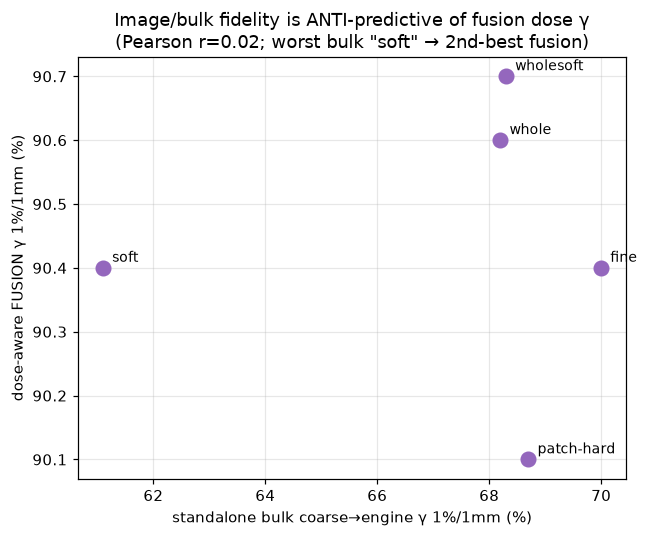
\includegraphics[width=.62\linewidth]{fig3_fidelity_antipredictive.png}
\caption{Image fidelity does not predict dose accuracy. Each point is one coarse-prior variant of the synthesis chain: \emph{soft} (soft-tissue-only bulk map), \emph{whole} (whole-image classifier), \emph{wholesoft} (whole-image classifier, soft-tissue bulk values), \emph{fine} (finer tissue classes), \emph{patch-hard} (patch-based classifier, hard labels). Horizontal axis: the variant's \emph{standalone} quality, the plan $\gam$1\%/1\,mm obtained when its bulk coarse CT is fed directly to the dose engine. Vertical axis: the \emph{fusion} accuracy, the plan $\gam$ of the full dose-aware pipeline built on that variant (jointly trained synthesizer $+$ dose network). Standalone quality spans 9 points but fusion accuracy varies by only 0.6 (Pearson $r{=}0.02$): the jointly trained refiner recovers dose-relevant density regardless of the coarse prior.}\label{fig:fidelity}\end{figure}

\begin{figure}[t]\centering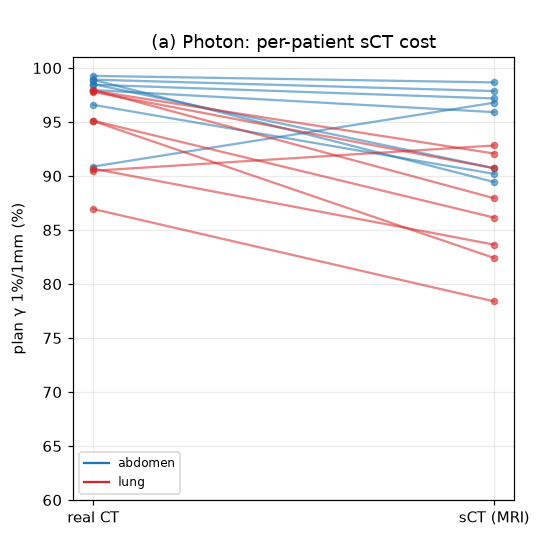
\includegraphics[width=.6\linewidth]{fig_sctcost_photonmri.png}
\caption{Per-patient synthesis cost on this task (real CT vs.\ sCT input, development fold; blue abdomen, red lung): photon drops are small and \emph{mixed}; photon dose is density-tolerant. The corresponding proton cost is $\sim$2$\times$ larger (see text).}\label{fig:cost}\end{figure}

\subsection{Diagnosing the hidden-test drop: MR intensity shift}
The gap between cross-validated (91.1) and hidden-test (84.1) gamma is itself a result worth
dissecting, because it is the failure mode every clinical MR-only deployment will face. Three
observations triangulate it. First, synthetically shifting our validation MRs (bias/gamma/scale
perturbations at magnitudes estimated from the test-set image statistics we could observe)
reproduced a drop of the observed size, and attributing it stage-by-stage placed most of it in
the shared tissue \emph{classifier}, not the refiner or dose network. Second, retraining the
classifier with strong intensity-shift augmentation recovered a substantial part of the board
drop on the sister proton-MRI task ($+3.1$ board gamma) and is deployed here. Third, the
recovery is partial and our synthetic shifts were harsher than the real ones, a calibration gap
we report so others can budget for it: internal shift probes over-predicted the recoverable
gain by roughly $4\times$. The residual hidden-test gap after augmentation is consistent with a
mixture of residual intensity shift and true anatomical distribution shift in the larger test
cohort.


\begin{figure}[t]\centering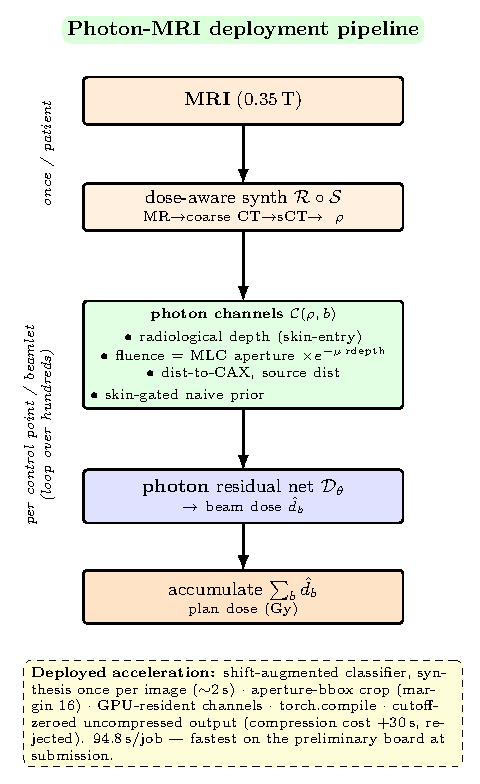
\includegraphics[width=.55\linewidth]{fig_deploy_photonmri.pdf}
\caption{The deployed Photon-MRI container: per patient, the density stage runs once; the
differentiable-channels $\to$ residual-net loop runs per control point/beamlet. The callout
lists the deployed acceleration measures and their measured effects.}\label{fig:deploy}\end{figure}

\subsection{Runtime engineering}
Runtime is double-weighted, and this submission held the fastest runtime on the preliminary
board at submission time (94.8\,s; the compressed-output variant of the same model ran 124.7\,s,
and margin 24 added a further $\sim$30\,s; both rejected by measurement). Photon-MRI adds one patient-level stage to the Photon-CT path; the
synthesizer runs once per source image ($\sim$2\,s, of which the two whole-image resamples and
two network forwards are profiled separately in the container log); after which the per-CP loop
is identical: aperture-bbox crops (margin 16, selected on full-grid metrics), GPU-resident
channels, compiled dose net, cutoff-zeroed uncompressed output (photon jobs are compute-bound;
an earlier compressed variant was $30$\,s slower). Two accuracy-relevant deployment details:
the naive prior at deploy is the same skin-entry-gated surrogate the network was trained with
(the CT container's build-up variant is \emph{not} interchangeable), and the whole-image
classifier requires the same inference mode as training, a sliding-window variant collapsed
lung on some grids in the sister proton container, a failure mode we gate for explicitly.



\begin{figure}[t]\centering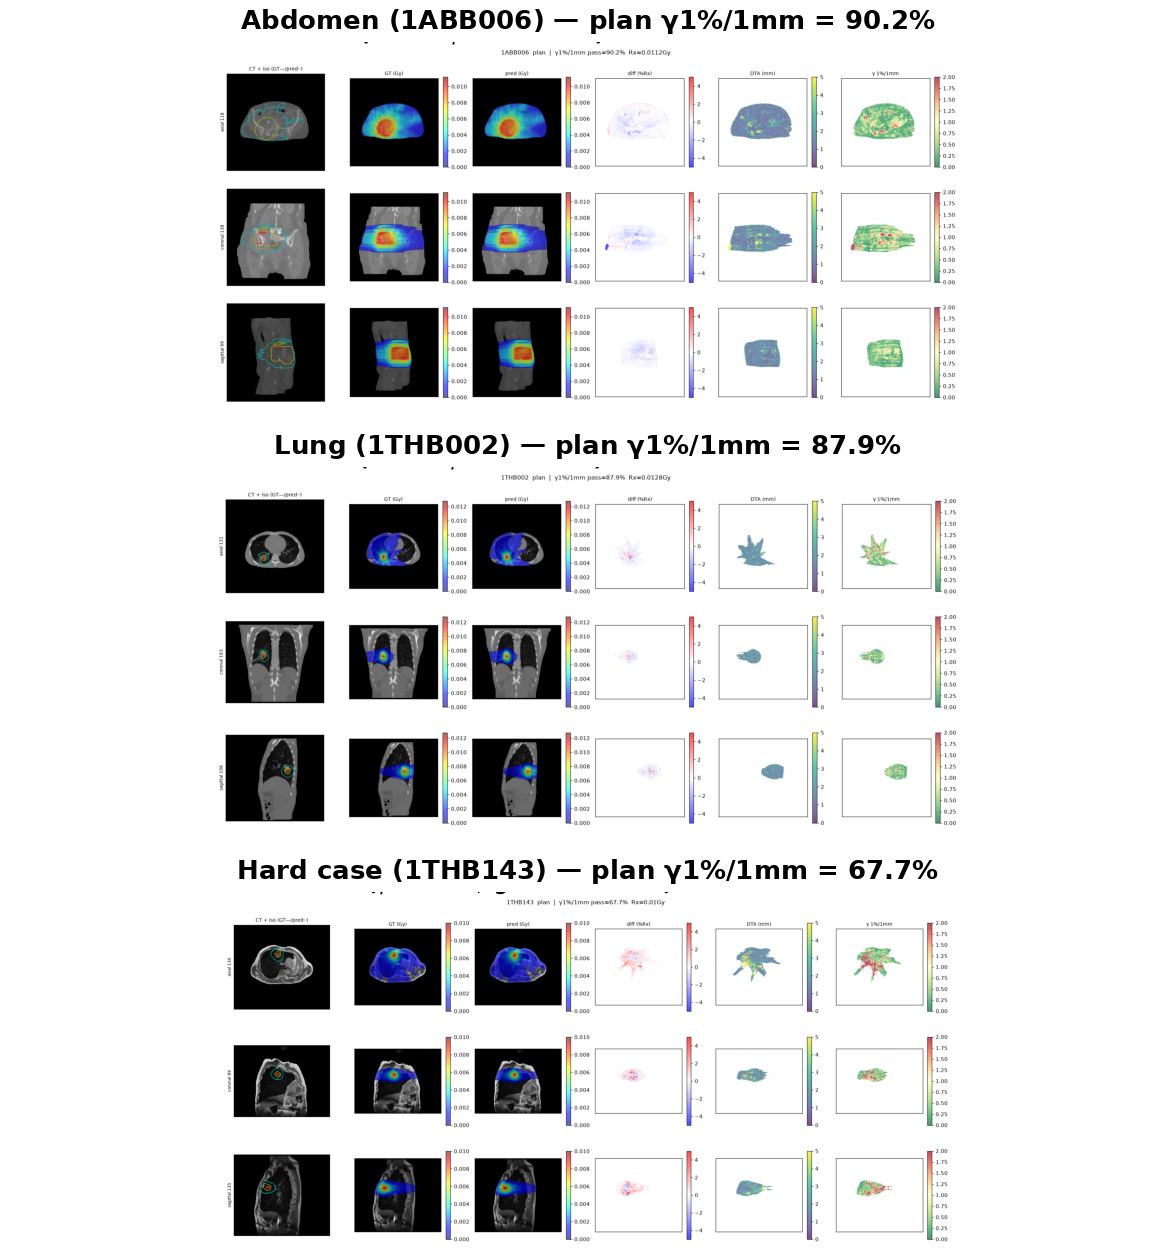
\includegraphics[width=.92\linewidth]{fig_qual_photonmri.png}
\caption{Qualitative Photon-MRI results on three cases spanning the difficulty range: abdomen (1ABB006, plan $\gam$1/1 $=90.2$), lung (1THB002, $87.9$), and the geometrically hard case 1THB143 ($67.7$; the worst patient in all four challenge tasks simultaneously, yet largely passing at 3\%/3\,mm: small-magnitude errors at steep lung--tissue interfaces). Columns: image with GT (solid) and predicted (dashed) isodose, MC dose, predicted dose, difference, distance-to-agreement, local $\gam$1\%/1\,mm.}\label{fig:qual}\end{figure}

\section{Discussion}
The central lesson of this task is that \emph{dose-aware synthesis works and image metrics
mislead}: +8.1 $\gam$ from bulk to learned sCT, +6.2 more from making synthesis serve the dose
(Table~\ref{tab:abl}), while image fidelity was non-predictive of the outcome ($r{=}0.02$). The
remaining gap to the real-CT ceiling ($4.7$ points cross-validated) is a genuine synthesis cost,
concentrated in lung at 0.35\,T where the MR simply carries little density information; better
segmentation and robustness augmentation both failed to close it, suggesting a data limit
(field strength, cohort size) rather than a capacity limit. \textbf{Limitations and
generalizability.} Single benchmark, single 0.35\,T scanner; the hidden-test intensity shift we
diagnosed is a preview of the cross-device shift any clinical deployment faces, and our
mitigation (shift-augmented classification) recovers only part of it. The ground truth is the
CT-computed dose mapped to the MR, so residual CT--MR registration error is label noise.
MR-linac photon planning with bulk or sCT densities is already clinically accepted; our
contribution is a stronger, dose-optimized MR-to-dose path and a caution about how to select
its components.

\emph{Why an intermediate sCT at all?} Three design questions deserve explicit answers.
First, the intermediate density image exists because it is the \emph{interface to the physics}:
the analytical operator (radiological depth, fluence attenuation) consumes a density map, and it
is this operator that supplies the residual-learning advantage and the data efficiency of the
whole framework; a direct MR-to-dose network would have to relearn that physics from 75
patients. Second, the synthesizer is partially transferred: the refiner is pretrained on 166
field-matched SynthRAD2025 MR--CT pairs before dose-aware joint training. Third, the dose-aware
sCT genuinely \emph{diverges} from an imaging-optimized sCT: trained through the dose loss, the
synthesizer accepts a worse image error where the dose does not need fidelity and spends its
capacity where the dose does; this is precisely why image fidelity stops predicting dose
accuracy (Sec.~3.3), and it means a dose-aware sCT should not be reused as a diagnostic-quality
image. Whether a fully sCT-free direct MR-to-dose model can match this pipeline remains open (we
did not run that controlled  experiment) and is our first future-work item.

\textbf{Future work.} (i) \emph{sCT-free direct MR-to-dose}: the fidelity result implies the
sCT is only a means to an end; a network consuming the MR (plus geometry channels computed on a
provisional density) end-to-end may bypass the synthesis bottleneck entirely, and the strongest
competing entries in this challenge appear to point the same way. (ii) \emph{Shift-robust
synthesis by design}: replace heuristic intensity augmentation with test-time
intensity-normalization or physics-based bSSFP signal modelling, targeting the classifier that
our attribution identified as the shift-sensitive stage. (iii) \emph{Speed}: our distilled
base-32 photon student (2.1$\times$, teacher-exceeding on CT) transfers to this task only after
finetuning on synthesis-domain channels, a domain-adapted student is trained and, if it passes
our no-accuracy-loss gate, halves the per-CP cost. (iv) \emph{Higher field and larger
cohorts}: the lung synthesis cost tracks the information limit of 0.35\,T bSSFP; 1.5\,T
MR-linac data is the clean test of how much of the remaining $4.7$-point ceiling gap is
physics rather than data.

\section{Author Contributions (CRediT)}
\textbf{Kai Wang:} Conceptualization, Methodology, Software, Validation, Formal analysis,
Investigation, Data curation, Writing -- original draft, Visualization.
\textbf{Meixu Chen:} Software (deployment and runtime optimization), Investigation
(acceleration study), Validation, Writing -- review \& editing.
\textbf{Rui Yang:} Conceptualization, Methodology, Writing -- review \& editing, Supervision.

\section{Other Information}
\textbf{Funding:} No external funding was received for this work.
\textbf{Collaborators:} None beyond the listed authors.
\textbf{Writing assistance:} Large-language-model assistance (Claude, Anthropic) was used in drafting and editing the text of this report; all methods, experiments, analyses and conclusions are the authors' own.
\textbf{Code availability:} The full implementation (models, differentiable physics operators,
deployment containers, and weights) will be released open-source at
\url{https://github.com/wangkaiwan/PhyPriorNet} before the challenge deadline (2026-10-01).

\clearpage
\begin{thebibliography}{9}\small
\bibitem{mriproton} Tian, L., et al.: MRI-based proton dose calculation for pelvic tumors using
deep learning. Phys. Med. Biol. \textbf{71}, 045003 (2026)
\bibitem{rsp} Gao, Y., et al.: MRI-only based material mass density and relative stopping power
estimation via deep learning for proton therapy. Sci. Rep. \textbf{14}, 11166 (2024)
\bibitem{liver} Liu, Y., et al.: MRI-based treatment planning for proton radiotherapy: dosimetric
validation of a deep-learning liver synthetic-CT method. Phys. Med. Biol. \textbf{64}, 145015 (2019)
\bibitem{ganbrain} Kazemifar, S., et al.: Dosimetric evaluation of synthetic CT generated with
GANs for MRI-only proton therapy planning of brain tumors. J. Appl. Clin. Med. Phys.
\textbf{21}(5), 76--86 (2020)
\bibitem{uncert} Li, X., et al.: Uncertainty-aware MR-based CT synthesis for robust proton therapy
planning of brain tumour. Radiother. Oncol. \textbf{189}, 109902 (2023)
\bibitem{dect} Liu, R., et al.: Synthetic dual-energy CT for MRI-only based proton therapy
treatment planning using label-GAN. Phys. Med. Biol. \textbf{66}, 065014 (2021)
\bibitem{totalsegmr} Wasserthal, J., et al.: TotalSegmentator MRI: robust sequence-independent
segmentation of anatomic structures in MRI. Radiology (2025)
\bibitem{gamma} Low, D.A., Harms, W.B., Mutic, S., Purdy, J.A.: A technique for the quantitative
evaluation of dose distributions. Med. Phys. \textbf{25}, 656--661 (1998)
\bibitem{matrad} Wieser, H.P., et al.: Development of the open-source dose calculation and
optimization toolkit matRad. Med. Phys. \textbf{44}, 2556--2568 (2017)
\bibitem{challenge} DoseRAD2026 Grand Challenge, \url{https://doserad2026.grand-challenge.org} (2026)
\bibitem{synthrad} Thummerer, A., et al.: SynthRAD2025 Grand Challenge dataset: generating
synthetic CTs for radiotherapy. Med. Phys. (2025)
\end{thebibliography}

\end{document}
